%% %%%%%%%%%%%%%%%%%%%%%%%%%%%%%%%%%%%%%%%%%%%%%%%%%%%%%%%%%%%%%%%%%%%%%%%%%%%
%%
%%          $Id: general_rules.tex 420 2013-04-08 15:30:35Z holz $
%%    author(s): RoboCupAtHome Technical Committee(s)
%%  description: description of the GENERAL RULES
%%
%% %%%%%%%%%%%%%%%%%%%%%%%%%%%%%%%%%%%%%%%%%%%%%%%%%%%%%%%%%%%%%%%%%%%%%%%%%%%
\chapter{General Rules \& Regulations}
\label{chap:rules}

These are the general rules and regulations for the competition in the RoboCup@Home league.
Every rule in this section can be considered to implicitly include the 
term \emph{``unless stated otherwise''}, meaning that additional or contrary rules in particular
test specifications have a higher priority than those mentioned herein in the general rules and regulations.  


\section{Team Registration and Qualification}


\subsection{Registration and Qualification Process}\label{rule:participation}

Each year there are four phases in the process toward participation:
\begin{enumerate}
\item \iterm{Intention of Participation} (optional)
\item \iterm{Preregistration} 
\item \iterm{Qualification} announcements
\item Final \iterm{Registration} for qualified teams
\end{enumerate}
Positions 1 and 2 will be announced by a call on the \iterm{RoboCup\char64Home mailing list}.
Preregistration requires a \iterm{team description paper}, a \Term{video}{qualification video} and a \Term{website}{Team Website}.

\subsection{Qualification Video}
As a proof of running hardware, each team has to provide a \iterm{qualification video}. 
As a minimum requirement for qualification, we consider showing the robot(s) successfully 
solving at least one test of the current or last year's rulebook.

\subsection{Team Website}

The \iterm{Team Website} has to contain photos and videos of the
robot(s), a description of the approaches, and information on
scientific achievements, relevant \iterm{publications}, team members,
and previous participation in RoboCup.

The information on the team website has to be in English and should be designed for a broader audience.

\subsection{Team Description Paper}\label{rule:website_tdp}
The \iaterm{team description paper}{TDP} should at least contain the following sections:
\begin{itemize}
\item Name of the team
\item contact information
\item website
\item team members
\item description of the hardware, including photo(s) of the robot(s)
\item description of the software
\end{itemize}

~\\\noindent Preferably, it should also contain the following:
\begin{itemize}
\item the focus of research and the contributions in the respective fields, 
\item innovative technology (if any), 
\item re-usability of the system for other research groups
\item applicability of the robot in the real world
\end{itemize}

~\\\noindent The TDP has to be in English, up to eight pages in length and formatted according to the guidelines of the RoboCup International Symposium.
It goes into detail about the technical and scientific approach.


%% %%%%%%%%%%%%%%%%%%%%%%%%%%%%%%%%%%%%%%%
\subsection{Qualification}
\label{rule:qualification}

During the \iterm{qualification process} a selection will be made by the 
%SVEN: before this was the OC not TC: 'technical committee' changed to OC.
organizing committee.
Taken into account and evaluated in this decision process are:
\begin{itemize}
\item The information on the team website and the qualification video,
\item the information in the \iterm{team description paper}, and
\item the information in the \iterm{RoboCup\char64Home Wiki} (added by the team).
\end{itemize}
(Additional) evaluation criteria are: 
\begin{itemize}
\item the performance in previous competitions, 
\item the relevant scientific contributions and publications, and
\item the contributions to the RoboCup@Home league.
\end{itemize}
For getting considered in the evaluation, be sure to insert your team's name 
when adding information to the \iterm{RoboCup\char64Home Wiki}.    




%% %%%%%%%%%%%%%%%%%%%%%%%%%%%%%%%%%%%%%%%%%%%%%%%%%%%%%%
\section{Scenario}
\label{sec:scenario}

The tests take place in the \iterm{RoboCup@Home arena}.
In addition, particular tests are situated outside the arena, e.g., in a previously unknown public place.
The following rules are related to the \iterm{RoboCup@Home arena} and its contents. 

\subsection{RoboCup@Home arena}
The \iterm{RoboCup@Home arena} is a realistic home setting consisting of 
inter-connected rooms like, for instance, a living room, a kitchen, a bath 
room, and a bed room. 

% \subsection{Team area}\label{rule:scenario_team_area}

% \todo{remove? does not depend on the rules, but on local organization }
% The maximum number of people to register per team is unlimited, but
% the organization only provides space for \emph{four} (4) persons to
% work at tables in the team area. 
% \todo{this is actually more an additional note for the registration information}

\subsection{Walls, doors and floor}\label{rule:scenario_walls}

The indoor home setting will be surrounded by high and low \Term{walls}{Arena walls}.
These walls will be built up using standard fair construction material.

\begin{enumerate}
{\bf\item Walls:} Walls have a minimum height of \SI{60}{\centi\meter}.
  A maximum height is not specified, but should be chosen so that the audience is able to watch the competition.\\
  Walls will be fixed and are likely to be not modified during the competition (see \refsec{rule:scenario_changes}). 
{\bf\item Doors:} There will be at least two entry/exit \Term{doors}{Arena doors} connecting the outside of the scenario.
  These doors are used as starting points for the robots (see \refsec{rule:start_position}).
  % At least one of the entrances will be a door with a handle (not a knob).\
  There will be also another door inside the scenario with a handle (not a knob) between any two rooms.
{\bf\item Floor:} The floor of the arena as well as the doorways of the arena are even.
  That is, there will be no significant steps or even stairways. 
  However, minor unevenness such as carpets, transitions in floor covering between different areas, 
  and minor gaps (especially at doorways) must be expected.
{\bf\item Appearance:} Floor and walls are mainly uni-colored but can 
  contain texture, e.g., a carpet on the floor, or a poster or picture 
  on the wall.\\
  Although being unlikely at the moment, transparent elements are also possible. 
\end{enumerate}


\subsection{Furniture}\label{rule:scenario_furniture}

The arena will be equipped with typical objects (furniture) that are
not specified in quantity and kind. 
The minimal configuration consists of 
\begin{itemize}
\item a small dinner table with two chairs, 
\item a couch, 
\item an open cupboard or small table with a television and remote control, 
\item a cupboard or shelf (with some books inside), and
\item a refrigerator in the kitchen (with some cans and plastic bottles inside). 
\end{itemize}
A typical arena setup is shown in \reffig{fig:scenario_arena}.

\begin{figure}[tbp]
  \centering
  \subfloat[Typical arena]{\label{fig:scenario_arena}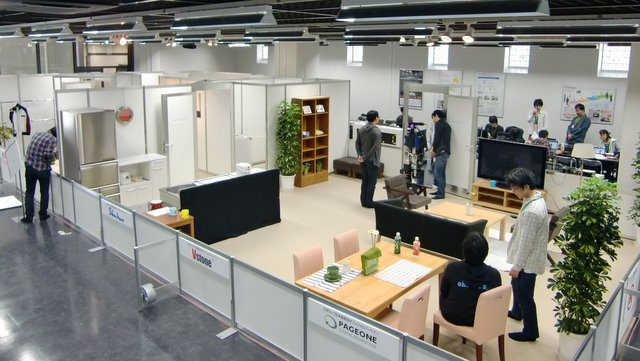
\includegraphics[height=46mm]{images/typical_arena.jpg}} ~ 
  \subfloat[Typical objects]{\label{fig:scenario_objects}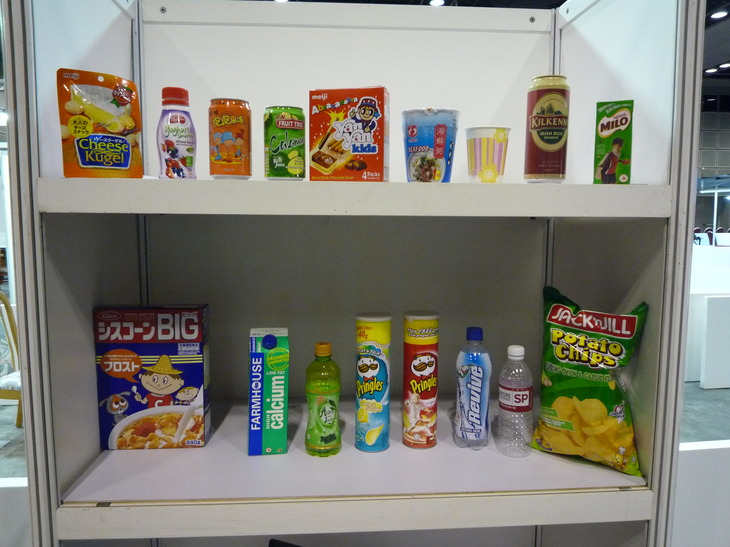
\includegraphics[height=46mm]{images/typical_objects.jpg}}
  \caption{Scenario examples: (a) a typical arena, and (b) typical objects.}
  \label{fig:arena}
\end{figure}



\subsection{Changes to the arena}\label{rule:scenario_changes}

Since the robots should be able to function in the real world the
scenario is not fixed and might change without further notice.
\begin{enumerate}
{\bf\item Major changes:} Changes will primarily influence the position of 
  objects such as furniture inside the arena while walls are likely to stay fixed.
  Multiple changes may take place up to completely restructuring the internals of the apartment. 
  The position of named locations (see \refsec{rule:scenario_names}) are not changed when used in a test, e.g., as navigation goal. \\
  In addition, passages may be blocked and cleared, respectively. 
  One hour before a test slot begins no \iterm{major changes} will be made.
{\bf\item Minor changes:} In contrast to major changes, \iterm{minor changes} like, 
  for instance, slightly moved chairs cannot be avoided and may happen at any time (even during a test). 
\end{enumerate}


\subsection{Predefined objects}\label{rule:scenario_objects}

\def\NumObjects{25\ }
\def\NumLocations{20\ }
\def\NumNames{20\ }

Some tests in the RoboCup@Home league involve the manipulation of objects. 
These objects resemble items usually found in household environments like, for instances, 
soda cans, coffee mugs or books. An example of objects used in a previous competition can be 
seen in \reffig{fig:scenario_objects}.

\begin{enumerate}
{\bf\item Definition:} The TC will compile a list of \NumObjects objects. 
  There are no restrictions on object size, appearance or weight. % (YES, this sentence is NOT NEW, but have been in the old rulebook!) 
  However, it can be expected that the selected objects are easily 
  manipulable by a human using a single hand.
{\bf\item Object classes:} Each object will be assigned to an \iterm{object class}.
  The objects 'lemonade' and 'ice tea' may be of class 'beverage' for example.
{\bf\item Object (class) locations:} Each object (class) will be assigned to an \iterm{object location}.
  Objects of class 'drink' may be usually found on the 'kitchen table' for example. 
{\bf\item Announcement:} The TC makes the set of objects (and their names, classes, and usual locations) available during the setup days.
{\bf\item Known vs.\ unknown}: These objects are used as the \iterm{known objects} in the test specifications;
  \iterm{unknown objects} are not taken from the set of \iterm{predefined objects}. 
{\bf\item Placement:}\nterm{object placement} In manipulation tasks, 
  the objects will be positioned at \iterm{manipulation locations} and less than \SI{15}{\centi\meter} away from the border of the surface 
  they are located at. 
  There will be at least 5cm space around each object.
\end{enumerate}



\subsection{Predefined locations}\label{rule:scenario_locations}

Some tests in the RoboCup@Home league involve \iterm{predefined locations}. 
These may include places like a 'bookshelf' or a 'dining table', as well as certain objects such as a 'television', or the 'front door'. 

\begin{enumerate}
{\bf\item Definition:} The TC will compile a list of predefined locations.
  There are no restrictions on which parts of the arena will be selected as a predefined location. 
{\bf\item Location classes:} Each location will be assigned to a \iterm{location class}. 
  The objects 'couch' and 'arm chair' may be of class 'seat' for example. 
{\bf\item Announcement:} The TC makes the set of locations (and their names and classes) available during the setup days.
{\bf\item Position:} The positions of locations are \emph{not} necessarily fixed (see \refsec{rule:scenario_changes}).
{\bf\item Manipulation locations:} The TC will mark \NumLocations locations out of the set of predefined locations as being \iterm{manipulation locations}.
Whenever a test involves manipulation, the object to manipulate will be placed 
at one of the manipulation locations. 
\end{enumerate}



\subsection{Predefined rooms}\label{rule:scenario_rooms}
Some tests in the RoboCup@Home league involve \iterm{predefined rooms}. 
\begin{enumerate}
{\bf\item Definition:} The TC will compile a list of room names.
{\bf\item Announcement:} The TC makes the set of rooms available during the setup days.
\end{enumerate}



\subsection{Predefined (person) names}\label{rule:scenario_names}

Some tests in the RoboCup@Home league involve \iterm{predefined names} of people. 

\begin{enumerate}
{\bf\item Definition:} The TC will compile a list of \NumNames predefined names.
  The names are \SI{50}{\percent} male and \SI{50}{\percent} female,
  and taken from the (current) most common first names in the United States.\\
  In order to ease speech recognition, it is tried to select names to be phonetically different from each other. 
{\bf\item Announcement:} The TC makes the set of names available during the setup days.
{\bf\item Assignment:} When a test involves interacting with persons (using a person's name),
  all involved persons are assigned names by the referees before the test. 
\end{enumerate}

Typical names are, for example, James, John, Robert, Michael and William as male names;
Mary, Patricia, Linda, Barbara and Elizabeth as female names.


%% %%%%%%%%%%%%%%%%%%%%%%%%
\subsection{Wireless network}\label{rule:scenario_wifi}

For wireless communication, an \iterm{arena network} is provided.
The actual infrastructure depends on the local organization. 

\begin{itemize}
\item To avoid interference with other leagues, this WIFI has to be used for communication only. 
  It is not allowed to use the above or any other WIFI network for personal use at the venue.
\item During the competitions, only the active team is allowed to use the \iterm{arena network}. 
\item The organizers cannot guarantee reliability and performance of wireless communication. 
Therefore, teams are required to be ready to setup, start their robots and run the tests even if, for any reason, network is not working properly.
\end{itemize}

% Preferably the organizers will try to provide one LAN cable on the
% desk of each participating team for Internet connection. However, this
% cannot be guaranteed. If multiple LAN connections are needed, each
% team has to bring its own LAN hub/switch and cables.

\subsection{Smart Home Devices}\label{rule:smarthomedevices}

\todo{Finish writing this section.}
There is a list of official devices that can be used in some tests for additional score.
The protocol to communicate with these devices will be provided well beforehand the
competition.


%%%%%%%%%%%%%%%%%%%%%%%%%%%%%%%%%%%%%%%%%%%%%%%%%%%%%%%%%%%%%%%%%%%%%%%%%%%%%%%
\section{Robots}\label{rule:robots}

\subsection{Autonomy \& Mobility}
Robots that participate in the RoboCup@Home league need to be
\Term{autonomous}{Autonomy} and \Term{mobile}{Mobility}.
Any deviations reported to the TC, may result in a penalty for the team (see \refsec{rule:extraordinary_penalties}).


\subsection{Number of robots}\label{rule:robots_number}

\begin{enumerate}
{\bf\item Registration:} The maximum \term{number of robots} per team that can be registered for the competitions is \emph{two} (2).
{\bf\item Regular Tests:} Only one robot is allowed per test. 
  For different tests different robots can be used.
{\bf\item Open Demonstrations:} In the Open Challenge and the Finals both robots can be used simultaneously.
{\bf\item RoboZoo:} In the RoboZoo both robots can be used simultaneously as long as they fit into the cage.
\end{enumerate}


\subsection{Size and weight of robots}\label{rule:robots_size}

\begin{enumerate}
{\bf\item Dimensions:} The dimensions of a robot should not exceed the limits of an average door, 
which is \SI{200}{\centi\meter} by \SI{70}{\centi\meter} in most countries.\\ 
The TC may allow the qualification and registration of larger robots, 
but due to the international character of the competition it cannot be guaranteed that the robots can actually enter the arena.  
In case of doubt, contact the local organization. 
{\bf\item Weight:} There is no specific weight restriction. 
However, the weight of the robot and the pressure it exerts on the floor should not exceed 
local regulations for the construction of buildings which are used for
living and/or offices in the country where the competitions is being held.
{\bf\item Transportation:} Team members are responsible for quickly moving the robot out of the arena. 
If the robot cannot move by itself (for any reason), the team members must 
be able to transport the robot away with an easy and fast procedure.
\end{enumerate}



\subsection{Emergency stop button}\label{rule:robots_emergency_button}

\begin{enumerate}
{\bf\item Accessibility and visibility:} Every robot has to provide an easily accessible and visible \iterm{emergency stop} button. 
{\bf\item Color:} It must be coloured red, and preferably be the only red button on the robot. 
If it is not the only red button, the TC may ask the team to tape over or remove the other red button. 
{\bf\item Robot behavior:} When pressing this button, the robot and all parts of it have to stop moving immediately.
{\bf\item Inspection:} The emergency stop button is tested during the \iterm{Robot Inspection} test (see \refsec{sec_robot_inspection}).
\end{enumerate}



\subsection{Start button}
\label{rule:start_button}

\begin{enumerate}
  {\bf\item Requirements:} As stated in \refsec{rule:start_signal}, teams that aren't able to carry out the default start signal (opening the door) have to provide a \iterm{start button} that can be used to start tests. The team needs to announce this to the TC before every test that involves a start signal, including \iterm{Robot Inspection}.
  {\bf\item Definition:} The start button can be any ``one-button procedure'' that can be easily executed by a referee.  This includes, for example, the release of the \iterm{emergency button} (\refsec{rule:robots_emergency_button}), a hardware button different from the \iterm{emergency button} (e.g., a green button), or a software button in a Graphical User Interface. 
  {\bf\item Inspection:} It is during the the \iterm{Robot Inspection} test (see \refsec{sec_robot_inspection}) that the procedure for the start button, if needed, is announced to the TC and inspected. The start button for a robot should be the same for all the tests.
  {\bf\item Penalty for using start button:} If a team needs to use the start button in a test where opening the door is the start signal, it may receive a penalty (see \refsec{rule:start_signal}).
\end{enumerate}



\subsection{Appearance and safety}\label{rule:roobt_appearance}

Robots should have a nice product-like appearance, be safe to operate and should not annoy its human users.
The following rules apply to all robots and are part of the \iterm{Robot Inspection} test (see \refsec{sec_robot_inspection}). 
\begin{enumerate}
{\bf\item Cover:} The robot's internal hardware (electronics and cables) should be covered in an appealing way.
The use of (visible) duct tape is strictly prohibited.
{\bf\item Loose cables:} There may not be any loose cables hanging out of the robot. 
{\bf\item Safety:} The robot may not have sharp edges or other things that could severe people.
{\bf\item Annoyance:} The robot should not permanently make loud noises or use blinding lights.
\end{enumerate}




\subsection{Audio output plug}\label{rule:roobt_audio_out}

\begin{enumerate}
{\bf\item Mandatory plug:} Either the robot or some external device connected to it \emph{must} have a \iterm{speaker output plug}. 
It is used to connect the robot to the sound system so that the audience and the referees can hear and follow the robot's speech output.
{\bf\item Inspection:} The output plug needs to be presented to the TC during the \iterm{Robot Inspection} test (see \refsec{sec_robot_inspection}).
{\bf\item Audio during tests:} Audio (and speech) output of the robot during a test have to be understood at least by the referees and the operators.
\begin{compactitem}
\item It is the responsibility of the teams to plug in the transmitter before a test, 
to check the sound system, 
and to hand over the transmitter to next team.
\item Do not rely on the sound system! 
For fail-safe operation and interacting with operators make sure that the sound system is not needed, e.g., 
by having additional speakers directly on the robot.
\end{compactitem}
\end{enumerate}

\section{External devices}\label{rule:roobt_external_devices}
\begin{enumerate}
{\bf\item Definition:} Everything which is not part of the robot is considered an \iterm{external device}. 
{\bf\item Inspection:} In general, external devices are not allowed unless presented and explained to the Technical Committee during the \iterm{Robot Inspection} test (see \refsec{sec_robot_inspection}).
{\bf\item Supervision:} In regular tests, external devices may only be used under supervision by referees and after approval by the TC. The devices have to be brought to the arena for every test, and removed quickly after the test.
{\bf\item Open demonstrations:} For the Open Challenge, RoboZoo, and the finals, external devices are allowed, still their use needs to be announced beforehand.
{\bf\item Wireless devices:} All \iterm{wireless devices} including bluetooth devices, walkie-talkies, and anything else that uses an RF signal to operate need to be announced to the \term{Organizing Committee (OC)}. The use of any wireless device not approved by the TC is strictly prohibited.  
{\bf\item Artificial landmarks:} \iterm{Artificial landmarks} and \iterm{markers} are not allowed.
{\bf\item Computing devices:} External computers for decentralized computations are allowed, but have to be inside the arena, i.e.,~not on its periphery.
{\bf\item Wireless LAN:} The use of networks other than the \iterm{arena network} (see \refsec{rule:scenario_wifi}) is strictly prohibited.
{\bf\item External microphones: }\iterm{External microphones}, hand microphones, and headsets are not allowed. Using an \iterm{on-board microphone} is mandatory for communication with the robot.
\end{enumerate}



\section{Organization of the competition}\label{sec:procedure_during_competition}

\subsection{Stage system}\label{rule:stages}

The competition features a \iterm{stage system}. 
It is organized in two stages each consisting of a number of specific tests. 
It ends with the finals.

\begin{enumerate}
{\bf\item Stage~I:} The first days of the competition will be called \iterm{Stage~I}. 
  All qualified teams can participate in Stage~I.
  Stage~I comprehends a set of \iterm{Ability Tests} and an \iterm{Integration Test}. Those \iterm{Proficency Tests} are performed at least 3 times each one.
  The \iterm{Open Challenge} is the open demonstration in Stage~I.

% MAURICIO: The advance schema changed. Also no demo challenge for 2015
%{\bf\item Stage~II:} The best \emph{50\% of teams}\footnote{If the total number of teams is less than 20, then the best 10 teams advance to Stage~II.} (after Stage~I) advance to \iterm{Stage~II}. 
%  Here, more complex abilities or combinations of abilities are tested. 
%  The \iterm{Demo Challenge} is the open---but scoped---demonstration in Stage~II.
{\bf\item Stage~II:} The best \emph{50\% of teams with full integrated capabilities}\footnote{If the total number of teams is less than 20, up to 10 teams may advance to Stage~II} (after Stage~I) advance to \iterm{Stage~II}. 
  Here, more complex abilities or combinations of abilities are tested. 
  In order to advance to Stage~II a team must successfully solve 3 out of 5 of the \iterm{Proficency Tests} in Stage~I
%  The \iterm{Open Challenge} is the open demonstration in Stage~II.
{\bf\item Final demonstration:} The best \emph{five teams} (after Stage~I and Stage~II) advance to the final round. 
  The final round features only a single open demonstration.
\end{enumerate}
% MAURICIO: No technical challenge for 2015
% In addition, a Technical Challenge (see \refsec{sec:TechnicalChallenge}) is carried out between Stage~II and the Final Demonstration, and its schedule is outside the scope of the Stage system.
In case of having no considerable score deviation between a team advancing to the next stage and a team dropping out, the TC may announce additional teams advancing to the next stage.


\subsection{Number of tests}\label{rule:number_of_tests}

\begin{enumerate}
\item In Stage~I, the \term{maximum number of tests} that a team can participate in is \emph{five (5)}.
\item In Stage~II, the \term{maximum number of tests} that a team can participate in is \emph{four (4)}.
\item None of the tests is mandatory, except for the \iterm{Robot Inspection} test (see \refsec{sec_robot_inspection}), the \iterm{Robo-Zoo} test (see \refsec{test:INTHOME}), and the \iterm{Basic Functionalities} test (see \refsec{test:BFPS}).
\item Teams have to indicate to the organizing committee in which tests they are going to participate. 
  Otherwise, they are automatically added to all test schedules and 
  may receive a penalty when not attending (see \refsec{rule:not_attending}).
\end{enumerate}


\subsection{Schedule}\label{rule:schedule}

\begin{enumerate}
{\bf\item Tests:} The organizing committee (OC) provides schedules for all tests and teams. 
{\bf\item Slots:} The tests will be held in \iterm{test slots} of approximately two hours.  
{\bf\item Preparation:} The organizing committee (OC) provides schedules for all teams to organize the access to the arena between test slots.
In these \iterm{preparation slots} the teams may conduct calibration procedures, remap the arena if necessary, or conduct test runs.
Preparation slots are inserted whenever possible, but may not be available before all test slots. 
{\bf\item Arena access:} One hour before a test slot, only the teams participating in that slot are allowed in the arena.
This rule only applies when not having organized \iterm{preparation slots}.   
\end{enumerate}


%\subsection{Score system}\label{rule:score_system}
%
%\begin{enumerate}
%  {\bf\item Stage~I:} The maximum total score per test in Stage~I is \scoring{2000 points}.
%  {\bf\item Stage~II:} The maximum total score per test in Stage~II is \scoring{2600 points}.
%  {\bf\item Special tests:} Tests may specify a maximum total score deviating from the general maximum total scores.  
%  {\bf\item Minimum score:} The minimum total score per test in Stage~I and Stage~II is \scoring{0 points}. 
%  That is, if the total score for a test is below zero, the team does not receive any points.
%  {\bf\item Penalties:} An exception to the \emph{minimum score} rule are penalties. 
%  Both penalties for not attending (see \refsec{rule:not_attending}) and extraordinary 
%  penalties (see \refsec{rule:extraordinary_penalties}) can cause a total negative score. 
%  {\bf\item Partial scores:} All tests---except for the open demonstrations---are rewarded on a partial scoring basis. 
%  \begin{enumerate}
%  \item Tests are split into designated parts.
%  \item Each part is assigned a certain number of points.
%  \item A team that successfully passes a designated part of the test receives points for that part.
%  \item In case of partial success, referees (and TC members) may decide to only award a percentage instead of the full partial score.  
%  \item The total score for a test is the sum of partial scores.
%  \item Partial scores can be negative (e.g.~to penalize failures etc.).
%  \end{enumerate}
%\end{enumerate}

% MAURICIO: Explained Score System
\subsection{Score system}\label{rule:score_system}

\begin{enumerate}
  {\bf\item Stage~I:} The maximum total score in Stage~I is \scoring{100 points}.
  \begin{enumerate}
    {\bf\item \iterm{Proficency Tests}:} The maximum total score is calculated as the average of the best two runs for that test
    {\bf\item RoboZoo:} The maximum score for RoboZoo is \scoring{5 points}.
  \end{enumerate}
  
  {\bf\item Stage~II:} Test in Stage~II are rewarded on a task-solved scoring basis.
  \begin{enumerate}
  \item Each test but the Open Challenge has a main task. The base score for solving the main task is \scoring{25 points}.
  \item The maximum score for Open Challenge is \scoring{20 points}.
  \item Optionals and subtasks add bonus points to the main task score.
  \end{enumerate}

  {\bf\item Finals:} Final score is normalized and special evaluation is used

  {\bf\item Special tests:} Tests may specify a maximum total score deviating from the general maximum total scores.
  {\bf\item Minimum score:} The minimum total score per test in Stage~I and Stage~II is \scoring{0 points}. That is, if the total score for a test is below zero, the team does not receive any points.
  {\bf\item Penalties:} An exception to the \emph{minimum score} rule are penalties. Both penalties for not attending (see \refsec{rule:not_attending}) and extraordinary penalties (see \refsec{rule:extraordinary_penalties}) can cause a total negative score. 
  {\bf\item Partial scores:} All tests---except for the open demonstrations---are rewarded on a partial scoring basis. 
  \begin{enumerate}
  \item Tests are split into designated parts.
  \item Each part is assigned a certain number of points.
  \item A team that successfully passes a designated part of the test receives points for that part.
  \item In case of partial success, referees (and TC members) may decide to only award a percentage instead of the full partial score.  
  \item The total score for a test is the sum of partial scores.
  \item Partial scores can be negative (e.g.~to penalize failures etc.).
  \end{enumerate}
\end{enumerate}


% MAURICIO: On 2015, Open Challenge may be moved to Stage 2. There is no Demo Challenge
\subsection{Open Demonstrations} \label{sec:open-demonstrations}
\begin{enumerate}
  {\bf\item Stage~I:} The \iterm{Open Challenge} is the open demonstration in Stage~I.
  \begin{enumerate}
  \item To participate in the Open Challenge, a team needs to participate in at least one regular Stage~I test.
  \item Teams can demonstrate freely chosen abilities. 
  \item The performance is evaluated by a jury consisting of the team leaders of all other teams.
  \item The Open Challenge is described in \refsec{sec:test_open_challenge}.
  \end{enumerate}
%  {\bf\item Stage~II:} The \iterm{Demo Challenge} is the open demonstration in Stage~II.
%  \begin{enumerate}
%  \item To participate in the Demo Challenge, a team needs to participate in at least one regular Stage~II test.
%  \item The scope (and topic) of the Demo Challenge are defined by the TC on a yearly basis.
%  \item Teams can demonstrate freely chosen abilities, but according to the scope. 
%  \item The performance is evaluated by the Technical Committee.
%  \item The Demo Challenge is described in \refsec{sec:test_demo_challenge}.
%  \end{enumerate}
  {\bf\item Finals:} The competition ends with a final demonstration.
  \begin{enumerate}
  \item The concept of the final demonstration is the same as that of the Open Challenge, but the performance evaluation is different. 
  \item The are two juries---an \emph{external} consisting of three or more people not from the RoboCup @Home league, and an \emph{internal} formed by the Executive Committee. Both juries have different sets of evaluation criteria.
  \item Members of the external jury are selected by the Executive Committee on site. 
  \item The demonstration in the finals does not have to be different from the one shown in the Open Challenge. It does not have to be the same either.
  \end{enumerate}
\end{enumerate}


\section{Procedure during Tests}

\subsection{Safety First!}\label{rule:safetyfirst}
\begin{enumerate}
{\bf\item Emergency Stop:} At any time when operating the robot inside and outside the 
  scenario the owners have to stop the robot immediately if there is a remote possibility 
  of dangerous behavior towards people and/or objects. 
{\bf\item Stopping on request:} If a referee, member of the Technical or Organizational 
  committee, an Executive or Trustee of the federation tells the team to stop the robot, 
  there will be no discussion and the robot has to be stopped \emph{immediately}.
{\bf\item Penalties:} If the team does not comply, the team and its members can be excluded 
  from the ongoing competition immediately by a decision of the RoboCup@Home Technical Committee. 
  Furthermore, the team and its members can be banned from future competitions for a period 
  not less than a year by a decision of the RoboCup Federation Trustee Board.
\end{enumerate}



\subsection{Maximum number of team members}\label{rule:number_of_people}
\begin{enumerate}
  {\bf\item Regular Tests:} During a regular test, the maximum number of team members allowed inside the arena is \emph{one} (1).
    The only exceptions are tests that require for more team members in the arena.
  {\bf\item Setup:} During the setup of a test, 
    the number of team members inside the arena is not limited. 
  {\bf\item Open Demonstrations:} During the Open Challenge, and the final demonstration, 
    the number of team members inside the arena is not limited. 
  {\bf\item Moderation:} During a regular test, one team member \emph{must} be available to host and comment the event (see \refsec{rule:moderator}).
\end{enumerate}



\subsection{Fair play}\label{rule:fairplay}
\iterm{Fair Play} and cooperative behavior is expected from all teams during the entire competition, in particular:
\begin{itemize}
\item while evaluating other teams, 
\item while refereeing, and 
\item when having to interact with other teams' robots.  
\end{itemize}
This also includes:
\begin{itemize}
\item not trying to cheat (e.g.~pretending autonomous behavior where there is none), 
\item not trying to exploit the rules (e.g.~not trying to solve the task but trying to score), and 
\item not trying to make other robots fail on purpose. 
\end{itemize}
Disregard of this rule can lead to penalties in the form of negative scores, and disqualification 
for a test or even for the entire competition. 

\subsection{Robot Autonomy and Remote Control}
\begin{enumerate}
{\bf\item No touching:} During a test, the participants are not allowed to make contact with the robot(s), 
  unless it is in a ``natural'' way and/or required by the test specification. 
{\bf\item Natural interaction:} The only allowed means to interact with the robot(s) are gestures and speech.
{\bf\item Natural commands:} Only general instructions are allowed. 
Anything that resembles direct control is prohibited.
 
{\bf\item Remote Control:} Remotely controlling the robot(s) is strictly prohibited. 
This also includes pressing buttons, or influencing sensors on purpose.
{\bf\item Penalties:} Disregard of these rules can lead to penalties in the form of negative scores, and disqualification 
for a test or even for the entire competition. 
\end{enumerate}

\subsection{Collisions}
\begin{enumerate}
  {\bf\item \iterm{Touching}:} Robots are allowed to gently \emph{touch} objects, items and humans. 
  They are not allowed to crash into something. 
  The "safety first" rule (\refsec{rule:safetyfirst}) supercedes all other rules.
  \begin{itemize}
   \item It \emph{is} allowed however to \emph{functionally} touch an item with e.g. the base.
  \end{itemize}
  The OC/TC/EC and the RoboCup Trustees all have the right to immediately stop a robot, and to disqualify a team for the 
  duration of the competition, or longer, in case of \emph{dangerous} behavior. 
  Furthermore, referees can recommend to disqualify a team in which case EC/TC decides.
  {\bf\item \iterm{Major collisions}:} If a robot crushes into something during a test, the robot is immediately stopped.
  Additional penalties may apply. 
  {\bf\item Robot-Robot avoidance:} If two robots encounter each other, they both have to actively try to avoid the other robot.
  \begin{enumerate}
  \item A robot which is not going for a different route 
    within a reasonable amount of time (e.g., \SI{30}{\second}) is removed.
  \item A non-moving robot blocking the path of another robot 
    for longer than a reasonable amount of time (e.g., \SI{30}{\second}) is removed.
    In this context, ``moving'' refers to any kind of motion or action required in the test. 
    For example, a robot standing still but manipulating an object does 
    not need to stop manipulating and move away, even when blocking the way
    of another robot for the duration of the manipulation.
  \end{enumerate}
\end{enumerate}



\subsection{Removal of robots}\label{rule:robot_removal}
Robots not obeying the rules are stopped and removed from the arena.
\begin{enumerate}
\item It is the decision of the referees and the TC member monitoring the test if and when to remove a robot.
\item When told to do so by the referees or the TC member monitoring the test, the team has to immediately stop the robot,
  and remove it from the arena without disturbing the ongoing test.
\end{enumerate}


\subsection{Start signal}\label{rule:start_signal}

\begin{enumerate}
  {\bf\item Opening the door:} Unless stated otherwise, the cue for the robot to enter the arena and start the test is the opening of the door by a referee.
  {\bf\item Start button:} If the robot is not able to automatically start after opening the door, the team may start the robot using a start button. 
  \begin{enumerate}
    \item Using a start button needs to be announced to the referees. It is the responsibility of the team to do so before the test starts.
    \item There may be penalties for using a start button in some tests
  \end{enumerate}
\end{enumerate}


\subsection{Entering and leaving the arena}\label{rule:start_position}
\begin{enumerate}
  {\bf\item Start position:} Unless stated otherwise, the robot starts outside of the arena.
  {\bf\item Entering:} The robot has to autonomously enter the arena.
  {\bf\item Success:} The robot is said to \emph{have entered} when the door used to enter can be closed again, and the robot is not blocking the passage.
\end{enumerate}



\subsection{Gestures}\label{rule:gestures}
Hand gestures may be used to control the robot in the following way:
\begin{enumerate}
{\bf\item Definition:} The teams define the hand gestures by themselves. 
{\bf\item Approval:} Gestures need to be approved by the referees and TC member monitoring the test.
Gestures should not involve more than the movement of both arms. 
This includes e.g.~expressions of sign language or pointing gestures.
{\bf\item Instructing operators:} It is the responsibility of the team to instruct operators.
\begin{enumerate}
\item The team may only instruct the operator when told to so by a referee.
\item The team may only instruct the operator in the presence of a referee.
\item The team may only instruct the robot for as long as allowed by the referee.
\item When the robot has to instruct the operator, it is the robot that instructs the operator and \emph{not} the team.
The team is not allowed to additionally guide the operator, e.g., tell the operator to come closer, speak louder, or to repeat a command.
\end{enumerate}
{\bf\item Receiving gestures:} Unless stated otherwise, it is not allowed to use 
a speech command to set the robot into a special mode for receiving gestures.
\end{enumerate}



\subsection{Referees}\label{rule:referees}
% \refmark{}
\begin{enumerate}
{\bf\item Setup:} Unless stated otherwise, each test is monitored by two referees and one member of the Technical Committee.
{\bf\item Selection:} The two referees 
\begin{itemize}
\item are chosen by EC/TC/OC, 
\item are announced together with the schedule for the test slot, 
\item and have to referee all teams in that slot.
\item Referees may not be from one of the teams in the slot.
\end{itemize}
{\bf\item Not showing up:} Not showing up for refereeing (on time) will result in a penalty (see \refsec{rule:extraordinary_penalties}). 
{\bf\item TC monitoring:} The referee from the TC acts as a main referee. 
{\bf\item Referee instructions:} Right before each test, referee instructions are conducted by the TC. The referees for all slots need to be present at the arena where the referee instructions are taking place.When and where referee instructions are taking place is announced together with the schedule for the slots.
\end{enumerate}


\subsection{Operator}\label{rule:operator}
\begin{enumerate}
{\bf\item Default operator:} The robots are operated by the monitoring TC member, 
a referee, or by a person selected by the TC.
{\bf\item Fallback/custom operator:} If the robot fails to understand the command given by the default operator, the team may continue with a custom operator.
\begin{compactitem}
\item The custom operator may be any person chosen by the team (and willing to do so); 
  including the referees or the monitoring TC member. 
\item A penalty may be involved when using a custom operator.
\end{compactitem}
\end{enumerate}

\subsection{Moderator}\label{rule:moderator}
\begin{enumerate}
{\bf\item Providing a moderator:} For each regular test (i.e., not for the open demonstrations), 
all participating teams need to provide a team member as moderator for the duration of their performance. 
{\bf\item Responsibilities:} The moderators have to:
  \begin{compactitem}
  \item explain the rules of the test, 
  \item comment on the performance of their team, 
  \item not interfere with the performance, 
  \item speak in English, 
  \item and obey the instructions by the monitoring TC member.
  \end{compactitem}
{\bf\item Competitive tests:} In competitive tests (tests in which two teams directly compete against each other),
the moderation has to be done by the two teams together.
\end{enumerate}


\subsection{Time limits}\label{rule:time_limits}
\begin{enumerate}
{\bf\item Stage~I:} Unless stated otherwise, the time limit for each test in Stage~I is \timing{5 minutes}.
{\bf\item Stage~II:} Unless stated otherwise, the time limit for each test in Stage~II is \timing{10 minutes}.
{\bf\item Setup time:} Unless stated otherwise, all time specifications, e.g., setup time and time for instructing operators, 
 are within the total test time. 
{\bf\item Scores:} When the time is up, the team has to immediately remove their robot(s) from the arena; no more points can be scored.
In special cases, the monitoring TC member may ask the team to continue the test for demonstration purposes (points cannot be scored). 
\end{enumerate}



\subsection{Restart}\label{rule:restart}
\begin{enumerate}
{\bf\item Number of restarts:} A team may request one (1) restart during a test, unless stated in otherwise.
There are tests in which a restart is not allowed.
{\bf\item Procedure:} In case a restart is allowed, the team may request the restart only before 50\% of the time alloted to the test.
The complete test is then restarted from the beginning (e.g., with entering the arena).  
The referees may rearrange the locations of objects/persons if necessary.
{\bf\item Time:} The time is neither restarted nor stopped. The team has 1 minute to restart the test (the same time to start the test); if the team is not able to do so in the allotted time, the test is called as finished by the TC.
{\bf\item Score:} The score of the second run (after the restart) counts. 
If it is lower than the score of the first run (before the restart),  
the average score of first and second run is taken.
{\bf\item Forced restart:} The referees and the monitoring TC member may force the team to do a restart:
\begin{compactitem}
  \item if the robot is doing nothing or nothing reasonable for \timing{one minute}, or
  \item when the robot fails to understand a command for \timing{five times}.
\end{compactitem}  
\end{enumerate}


\subsection{Bypassing Automatic Speech Recognition: Continue}\label{rule:asrcontinue}

Giving commands to the robot is an important part of many tests.
RoboCup@Home fosters natural human-robot interaction through gestures and speech, such that speech is the primary modality to give complex commands to the robot.
Due to the sequential nature of many tests and the difficulty of ASR in the international competition environment of RoboCup,
the team is allowed to take up to 2 alternative means to provide a command to the robot, for which the robot continuously fails to recognize the spoken command.
These alternative means should be declared in the registration form and checked by the TC during the \iterm{Robot Inspection} test (see \refsec{sec_robot_inspection}).

In future competitions, this rule will be gradually removed. 
Hence, solutions are encouraged that either resolve the ASR failure through spoken dialogues or solving the task in an alternative way (no penalty), or that use appealing modalities to provide the command (less penalty than direct typing on the robot).

\begin{enumerate}
{\bf\item Number of Continue's:} The team leader may request up to two (2) Continue's during a test. 
{\bf\item Procedure:} In case a Continue is allowed, the team may request the Continue only at moments in which the robot is failing at carrying out ASR (no pre-emptive Continue's are allowed).
A TC member gives the command through the alternative input modality. S/he provides exactly what the user has spoken. 
The Continue rule will not be allowed, if the robot does not have a keyboard attached or the alternative input modality was not accepted by the TC, or if it is not able to process ASR commands and alternative commands simultaneously.
{\bf\item Time:} The time is neither restarted nor stopped while the Continue rule is applied.
{\bf\item Score:} If one Continue was asked for, the points provided for the ASR part of the test (if any) will be zero and the total points for the test will be multiplied by a factor of 0.5 if the modality of the alternative solution is by typing on a keyboard. To promote other means of interaction, if the modality is different than keyboard typing (i.e. touch interface), the factor to be applied will be 0.75. If two Continues were asked for, the factor will be applied twice.
\end{enumerate}

\subsubsection{Alternative methods}
Below are some suggested alternatives for ASR:
\begin{itemize}
 \item A QR code encoding a text is shown to the robot on a laptop screen.
 \item The robot hosts a website on which some text can be entered.
 \item A laptop connects to the robot over e.g. ssh where some command can be entered. 
 \item ...
\end{itemize}




\section{Special penalties and bonuses}\label{sec:special_awards}


\subsection{Penalty for not attending}\label{rule:not_attending}
\begin{enumerate}
{\bf\item Automatic schedule:} All teams are automatically scheduled for all tests.
{\bf\item Announcement:} If a team cannot participate in a test (for any reason),
the team leader has to announce this to the OC at least \timing{60 minutes} before the test slot begins.
{\bf\item Penalties:} A team that is not present at the start position when their scheduled test starts, the team is not allowed to participate in the test anymore. If the team has not announced that it is not going to participate, it gets a penalty of \scoring{500 points}. 
\end{enumerate}

\subsection{Extraordinary penalties}\label{rule:extraordinary_penalties}
\begin{enumerate}
{\bf\item Penalty for inoperative robots:} If a team starts a test, but it does not solve any of the partial tasks
(and is obviously not trying to do so), a penalty of \scoring{-100 points} is handed out. 
The decision is made by the referees and the monitoring TC member.  
{\bf\item Extra penalty for collision:} In case of major, (grossly) negligent collisions the TC may disqualify the team for 
a test (the team receives \scoring{0 points}), or for the entire competition.
{\bf\item Not showing up as referee or jury member:}
If a team does not provide a referee or jury member (being at the arena on time), the team receives a penalty
of \scoring{500 points}, and will be remembered for qualification decisions in future competitions.\\
Jury members missing a performance to evaluate are excluded from the jury, and the team is 
disqualified from the challenge (receives \scoring{0 points}).
\end{enumerate}

\subsection{Bonus for outstanding performance}\label{rule:outstanding_performance}
\begin{enumerate}
\item For every regular test in Stage~I and Stage~II, the @Home Technical
Committee can decide to give an extra bonus for \iterm{outstanding performance} 
of up to 10\% of the maximum test score. 
\item This is to reward teams that do more than what is needed to solely score points in a
test but show innovative and general approaches to enhance the scope of @Home. 
\item If a team thinks that it deserves this bonus, it should announce (and briefly explain) 
this to the Technical Committee beforehand.
\item It is the decision of the TC if (and to which degree) the bonus score is granted.
\end{enumerate}


\section{Best Test Score Certificate}\label{sec:best_score_certificate}
A certificate will be given to the team with the highest score in each test of Stage 1 and 2. 

\begin{enumerate}
{\bf\item Requirements:} The score obtained must be at least 70\% of the maximum score of the test.
\end{enumerate}
% Local Variables:
% TeX-master: "../../rulebook"
% End:

\section{General Instructions for Organizing Committee}\label{sec:oc_general_instructions}
Although there are instructions for the OC are specified per test, there are several aspects that the OC requires to carry out for competition in general:
\begin{description}
\item[During competition:] \hfill
\begin{compactitem}
\item Provide TC and referees with scoring sheets, pens, clipboards, stopwatches and other material relevant of carrying out the scoring.
\item Post time schedules in the allotted spaces for the team's knowledge.
\end{compactitem}
\item[1h before each test:] \hfill
\begin{compactitem}
\item Organize referees.
\end{compactitem}
\end{description}


